
\documentclass[journal]{IEEEtran}

\usepackage{epsfig,graphicx,lineno,amssymb,mdwmath,array,amsmath}
% \usepackage{subfigure}
\usepackage{multirow}
\usepackage{xcolor}
\usepackage{cite}
\usepackage{epstopdf}
\usepackage{latexsym, bm}
\usepackage{algorithm}
\usepackage{algorithmicx}
\usepackage{algpseudocode}
\usepackage[utf8]{inputenc}
\usepackage[T1]{fontenc}
\usepackage{listings}

\usepackage[font=footnotesize]{subfig}
\usepackage{stfloats}


\definecolor{pblue}{rgb}{0.13,0.13,1}
\definecolor{pgreen}{rgb}{0,0.5,0}
\definecolor{pred}{rgb}{0.9,0,0}
\definecolor{pgrey}{rgb}{0.46,0.45,0.48}
\lstset{
  language=Java,
  frame=single,
  emph={enableRssiPolling},
%   emphstyle=\textbf,
  emphstyle=\color{red},
  showspaces=false,
  showtabs=false,
  breaklines=true,
  showstringspaces=false,
  breakatwhitespace=true,
  commentstyle=\color{pgreen},
  keywordstyle=\color{pblue},
  stringstyle=\color{pred},
%   basicstyle=\ttfamily,
  basicstyle=\small,
  stringstyle=\ttfamily,
  moredelim=[il][\textcolor{pgrey}]{$1$},
  moredelim=[is][\textcolor{pgrey}]{\%\%}{\%\%},
  numbers=left, numberstyle=\tiny, stepnumber=1, numbersep=5pt
}


\newtheorem{mydef}{Definition}
\newtheorem{mylem}{Lemma}
\newtheorem{mythm}{Theorem}
\newtheorem{cor}{Corollary}

\hyphenation{op-tical net-works semi-conduc-tor}

\makeatletter       %for algorithm
\def\BState{\State\hskip-\ALG@thistlm} %for algorithm
\makeatother %for algorithm

\algnewcommand\algorithmicswitch{\textbf{switch}}
\algnewcommand\algorithmiccase{\textbf{case}}

\algblockdefx[Name1]{SWITCH}{ENDSWITCH}%
%   [1]{\textbf{switch} #1 \textbf{do}}%
 [1]{\textbf{switch} #1}%
  {\textbf{end switch}}
\algblockdefx[Name2]{CASE}{ENDCASE}%
  [1]{\textbf{case} #1 \textbf{do}}%
  {\textbf{end case}}

\begin{document}
%
% paper title
% can use linebreaks \\ within to get better formatting as desired
% Do not put math or special symbols in the title.
\title{An Rssi-Aware Wi-Fi Download Management Approach for Energy Saving on Smartphones}
%
\author{Lunde~Chen,
        ~Huan~Li*,~\IEEEmembership{Member,~IEEE}% <-this % stops a space
\thanks{*Corresponding Author: H. Li,  is with the School
of Computer Science and Engineering, Beihang University, Beijing,
China 100191.
% ,  e-mail: lihuan@buaa.edu.cn
}% <-this % stops a space
\thanks{L. Chen is with with the School of Computer Science and Engineering and Ecole Centrale de P\'{e}kin, Beihang University, Beijing, China 100191.}
% <-this % stops a space
\thanks{Manuscript received October 5, 2014.}}

% The paper headers
\markboth{IEEE EMBEDDED SYSTEMS LETTERS}%%Journal of \LaTeX\ Class Files,~Vol.~11, No.~4, December~2012}%
{Shell \MakeLowercase{\textit{et al.}}: Bare Demo of IEEEtran.cls for Journals}

\maketitle

\begin{abstract}
Smartphones are emerging as a particularly appealing platform for network applications, 
especially through Wi-Fi interface. However,
Wi-Fi entails considerable energy consumption and smartphones
are bottlenecked by their battery capacity. Finding ways to reduce 
energy consumption of Wi-Fi is more than critical.
In this letter, we address the problem of energy saving of Wi-Fi 
with regarding to Rssi. Through extensive experiments, we investigate how 
Rssi influences energy consumption. Based on our experimental findings, 
we propose an Rssi-aware Wi-Fi download management approach for energy saving on smartphones.
Simulations show that our approach is effective and can achieve more than 100\% energy saving, 
both in a constantly moving scenario and in a stationary-moving scenario.
\end{abstract}

% Note that keywords are not normally used for peerreview papers.
\begin{IEEEkeywords}
Rssi, Energy saving, algorithm.
\end{IEEEkeywords}

\IEEEpeerreviewmaketitle

\section{Introduction}

% \IEEEPARstart{G}{uidance}: This paragraph is to address 1) the growth of the multimedia applications on smartphone 
% [Need some data evidence],
% and most need download large files, e.g., app tar files and movies etc.
% 2) the wifi access requirements for those applications, and 
% 3) major Wifi properties and the impact on the critical energy issues on resource-constrained smartphones. 
% {[\bf Guidance:]}  
% 1) The most widely used energy-efficient wifi access strategies, such as prediction sleeping methods are introduced here, 
% 2) The limits or problems of those strategies.
\IEEEPARstart{S}{martphones} are becoming increasingly popular and have emerged as a particularly appealing platform for network applications, 
especially through Wi-Fi interface.
However, these light-weighted and easy-to-carry mobile devices are constrained by their limited battery capacity.
We consider the scenario where people use their smartphones to download large files such as movies, documents and apk files.
Those files are typically 
larger than 10 MB and may take several minutes to complete the download.
The key challenge here is how to perform the download activity in an energy-efficient way so that 
it will not affect other applications. 

We investigate the relationship between the energy consumption and Rssi and conclude that Rssi has a major 
impact on the energy consumption. Downloading one file
in weak Rssi environment can consume 8 times more energy than in strong Rssi. Therefore, 
an Rssi-based Wi-Fi download management scheme is needed to achieve good energy efficiency.
% The ideal is to download files where Wi-Fi signal is strong and stable. 
However, on the one hand,
smartphones are naturally for mobile usage, resulting in a constantly changing Rssi environment.
On the other hand, even when the smartphone is stationary, Rssi is not stable and
demonstrates considerable fluctuations \cite{biblio1}\cite{biblio2}.

In this letter, we propose a scheme that can perceive the varying Rssi and automatically 
adjust the download actions. We conduct evaluation of our scheme using simulations.

\section{Evaluation of Rssi and Energy Consumption}
\subsection{Experimental Setup for Power Measurement}
The DUT (Device Under Test) 
is a Huawei 8950D running Android 4.0, equiped with a double-core 1.2GHz Snapdragon CPU and 768MB RAM, supporting IEEE 802.11 n/b/g.
We use a Monsoon Power Monitor \cite{biblio5} for power measurement.
The Monsoon Power Monitor supplies a stable voltage of 3.7V to the DUT and samples the power consumption at a rate of 5KHz. 

To perform the download, we developed an application using the DownloadManager\footnote[1]{DownloadManager is a
system service of Android that handles long-running HTTP downloads.} provided by Android. 
We also cross compiled Iptables and Tcpdump and installed them into the DUT as local libararies.
Iptables is used to block the Internet access of all applications 
except that of the download application so that no interference traffic is introduced. 
During the downloading time, the screen is off and WifiLock\footnote[2]{WifiLock allows to keep the Wi-Fi radio awake.}
is aquired. 
We measure the power consumed for 
completing downloading a file of 11.4MB, since the typical size of an apk file is about 10MB. 
% After this, we perform the same download at the same fixed location, but with Tcpdump running to dump traffic information. 
Each measurement is repeated 3 times. After that, we move the instruments to 
another location where Rssi is different and repeat the experiment. 
\subsection{Measurement Results}
%Put the figures and analysis here.
%\\
%\indent 
\begin{figure}
\centering
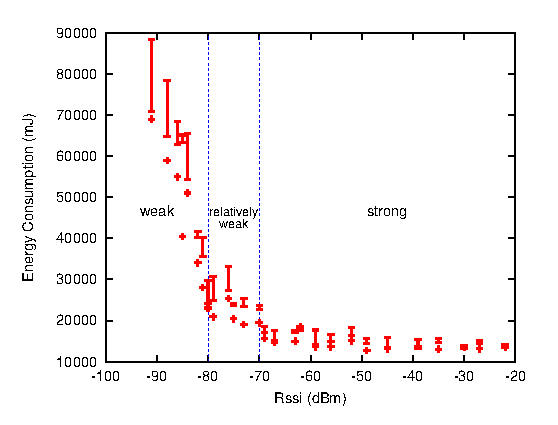
\includegraphics[scale=0.95]{rssi_energy.eps}
\caption{Energy Consumption in different Rssi}
\label{rssi_energy}
\end{figure}

Figure \ref{rssi_energy} shows the relationship between Rssi and the energy consumption. 
We can see that when Rssi is higher than -70dBm, 
the energy consumption for the download is limited and independent of Rssi.
When Rssi is between -80dBm and -70dBm, the energy consumption for the download increases as Rssi becomes weaker, but not so significantly.  
When Rssi is below -80dBm, the energy consumption for downloading files increases dramatically.
There is a clear threshold-based relationship between 
the Rssi and the energy consumption. 

Figure \ref{energy_throughtput_30dbm} and Figure \ref{energy_throughtput_84dbm} show the measured power for downloading
a file in strong (-30 dBm) and weak (-84 dBm) Rssi and the corresponding traffic throughputs.
% The measured power is mainly in the range of [250mA, 300mA] in strong Rssi and 
% in the range of [200mA, 250mA] in weak Rssi.
While the measured power is slightly higher in strong Rssi than in weak Rssi,
the throughput in strong Rssi is more than 5 times higher than in weak Rssi (1006KB/s vs 183KB/s).
So the total time for completing the download in strong 
Rssi is only 1/5 as in weak Rssi (11.4s vs 64s), which results 
in much smaller value in energy consumption (13312mJ vs 54397mJ).

% if error, type << pdflatex --shell-escape Version-2.tex >> in Terminal

\begin{figure}
\centering
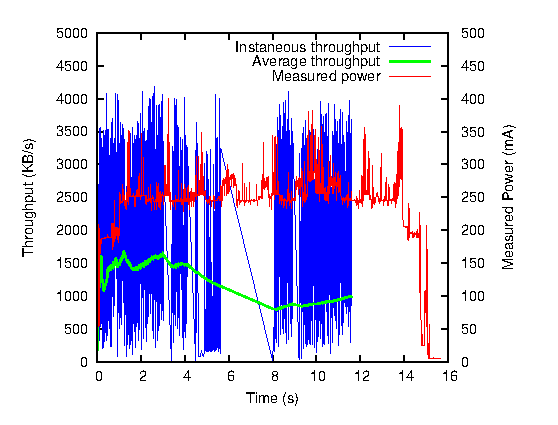
\includegraphics[scale=0.95]{energy_throughtput_30dbm.eps}
\caption{Measured power vs throughput and Rssi (-30dBm)}
\label{energy_throughtput_30dbm}
\end{figure}

\begin{figure}
\centering
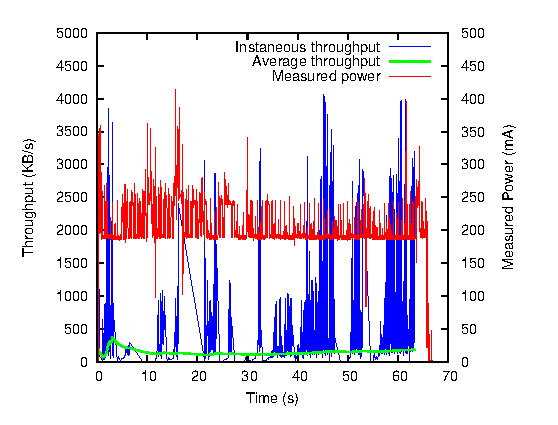
\includegraphics[scale=0.95]{energy_throughtput_84dbm.eps}
\caption{Measured power vs throughput and Rssi (-84dBm)}
\label{energy_throughtput_84dbm}
\end{figure}

As we can see in Figure \ref{energy_throughtput_30dbm} and Figure \ref{energy_throughtput_84dbm}, 
when the download is finished, Wi-Fi interface will continue to consume energy for 3-5 seconds.
We have the same observation when downloading small files (in the order of 10KB and of 100KB) and when stopping downloading files.
Our analysis using Tcpdump shows that the extra 3-5 seconds of energy consumption
is caused by the closure of TCP connection, as illustrated in Figure \ref{tail_energy}. 
We conclude that downloading files via Wi-Fi introduces
significant tail energy when stopping or finishing a download.
Althrough existing researches have been done for the tail energy of celullar networks \cite{biblio6},
this is the first time that the tail energy phenomenon in Wi-Fi environment
is observed and investigated.
We can see that tail energy represents a great overhead if the download session is short.

\begin{figure}
\centering
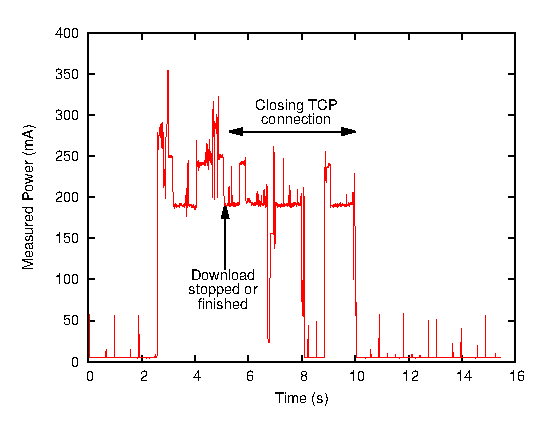
\includegraphics[scale=0.95]{tail_energy.eps}
\caption{Tail energy due to the closure of TCP connection when stopping or finishing a download}
\label{tail_energy}
\end{figure}

\section{Rssi-based Wi-Fi Download Management Algorithm}
As Rssi has a significant impact on the energy consumption of file downloading in Wi-Fi environment, one may consider closing Wi-Fi interface 
when Wi-Fi signal is becoming weak and reopening it when Wi-Fi signal is becoming strong \cite{biblio7}. However, our experiments show that 
closing and openning Wi-Fi interface consumes much energy, i.e. 3700 mJ and 4300 mJ respectively, as shown in Figure \ref{energy_open_close_wifi}. 
Keeping Wi-Fi interface open, on the other hand, consumes only 3.95 mW overhead. 
As the result, the energy consumption of closing and openning Wi-Fi interface 
is equal to that of keeping Wi-Fi interface open for 2025 seconds.
Besides, keeping Wi-Fi interface open allows to monitor Wi-Fi condition and adjust the smartphone's networking behaviors accordingly.
To this end, in designing our Rssi-based download management algorithm, we keep Wi-Fi interface open.

According to the experimental results,
we divide Rssi of Wi-Fi into 3 status: strong, relatively weak and weak, 
based on its impact on energy consumption. Accordingly, 
we define 3 different states of Wi-Fi: \textit{good}, \textit{unknown} and \textit{bad}. 
The transition among the three states is illustrated as a Finite State Machine (FSM) in Figure \ref{FSM}. 
At each iteration, the current state of Wi-Fi is updated according to the status of Rssi.

\begin{figure}
\centering
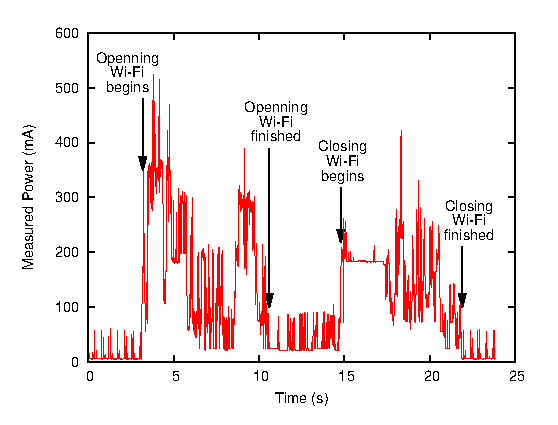
\includegraphics[scale=0.95]{energy_open_close_wifi.eps}
\caption{Measured power for openning and closing Wi-Fi interface}
\label{energy_open_close_wifi}
\end{figure}

\begin{figure}
\centering
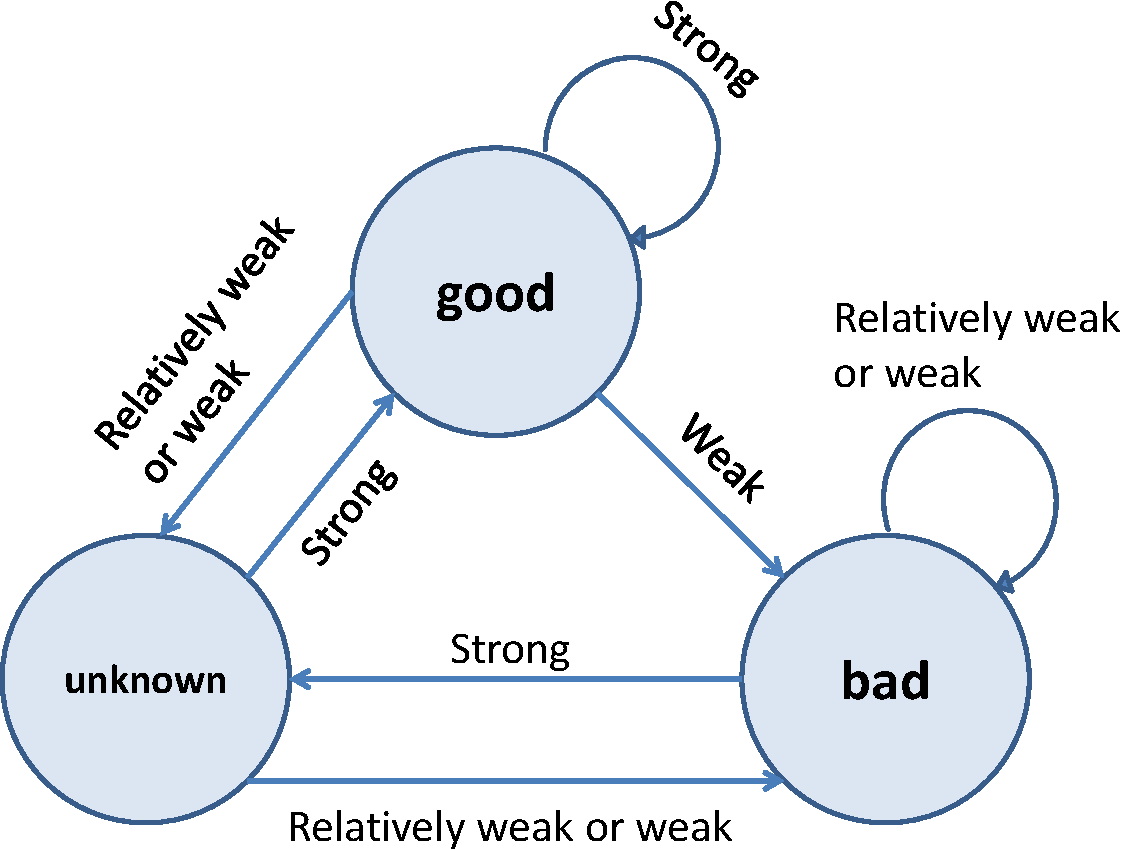
\includegraphics[scale=0.35]{FSM.pdf}
\caption{FSM for updating current state of Wi-Fi}
\label{FSM}
\end{figure}

The basic idea 
is to start downloading files when the state of Wi-Fi is \textit{good}, and to stop downloading files when the state is \textit{bad}. If the state 
is \textit{unknown}, 
no action will be taken.
The pseudo-code of the Rssi-aware download management algorithm is given in Algorithm 1.

\begin{algorithm}
\caption{Rssi-based Download Management Algorithm}\label{rssi_algorithm}
\begin{algorithmic}[1]
\While {true}
\State /*Update current state of Wi-Fi,  
\State  *as shown in Figure \ref{FSM} */
\State curr\_state $\gets$ update\_state(prev\_state, rssi\_measured)
\If {curr\_state is \textit{good}}
\State start\_download()
\ElsIf {curr\_state is \textit{bad}}
\State stop\_download()
\EndIf
\State prev\_state $\gets$ curr\_state
\State sleep() //sleep for 1 second
\EndWhile
\end{algorithmic}
\end{algorithm}

The main purpose of our algorithm is to leverage the varying nature of Rssi. 
As each measurement could introduce inaccuracy, Wi-Fi state \textit{unknown}
is set so as to leave the decision-making in the next iteration when 
it is not certain whether the change of Rssi is due to the smartphone user moving or due to
the fluctuations of Rssi itself.
In this way, we avoid constantly starting and stopping downloads.
This is effective because the relationship between Rssi and energy consumption is threshold-based, 
and thus the delay of 1 second in decision-making is tolerable.

The algorithm is light-weighted and causes negligible energy overhead during the running time. 
On the one hand, we simply need to store the Wi-Fi state of the previous iteration
and each decision-making takes only O(1) computation.
On the other hand, the Rssi calculation is done by the Android OS and WifiService\footnote[1]{WifiService and 
SystemServer are system services of Android.}
and can be obtained through API provided by WifiManager\footnote[2]{WifiManager is an Android API for managing Wi-Fi connectivity.}.
In fact, once Wi-Fi is connected to an AP, 
WifiService will be started in SystemServer
and Rssi will be calculated periodically.
We implemente our algorithm as an application.
The energy overhead of running the application 
cannot be measured because it's too insignificant, far less than 0.001mA. 
Therefore, we can consider the energy overhead of our algorithm
as zero.


\section{Simulation Results}
In this section, we present the Monte Carlo 
simulation of the Rssi-aware Wi-Fi download
management approach and the simulation results.
\subsection{Simulation Methodology}
{\bf User's Moving Behavior Model}: 
We model the moving behavior of a smartphone user as a directional random walk, 
which is defined as:
$$ s_{k_{t}} \sim \textrm{U}(s_{min}, s_{max}) \eqno(1) $$
$$ \theta_{k_{t}} \sim \textrm{N}(\theta_{k_{t-1}}, \sigma^2) \eqno(2) $$
where $s_{k_{t}}$ and $\theta_{k_{t}}$ are the speed and the heading of the smartphone user at instant $t$.

To simulate all possible starting point that the user could take, 
a 2-dimensional Halton sequence \cite{biblio8} with base \{2, 3\} is generated. 
When the user gets out of the signal range of Wi-Fi AP, we consider one walk is terminated and take the next value of the Halton sequence 
as his new starting point. This process is characterized as Equation (4), where $R$ refers to the radius of the signal range of Wi-Fi AP:
\[ \vec{P}_{k_{t=0}} = R\textrm{H}_{k}(2, 3) \eqno(4) \]

Considering that the user may use his phone not only on move, but also when he 
is stationary, we introduce a Markov chain to characterize this stationary-moving transition,
with two state spaces \textit{moving} and \textit{stationary}, represented by $\delta = $ 1 and  $\delta = $ 0.
We denote $p_{m}$ as the probability for the user keeping moving the next instant if he is on move at current instant, and 
$p_{s}$ as the probability for the user staying stationary if he is stationary at current instant. 
Then the position of the user
at next instant can be given as:
\[ \vec{P}_{k_{t+1}} = \vec{P}_{k_{t}} + \delta_{k_{t+1}}(p_{m}, p_{s})s_{k_{t}}{\cos\theta_{k_{t}} \choose \sin\theta_{k_{t}}} \eqno(5) \]

{\bf Rssi Variation Model}:
We adopt the logarithmic wireless path model \cite{biblio9} to calculate the real Rssi of Wi-Fi from the distance between the AP and the smartphone:
$$ Rssi(d) = Rssi(d0) + 10\eta\log(d/d0) + \xi \eqno(4)$$
where d0 is the reference distance, typically 1 meter, $\eta$ is the path attenuation factor and $\xi$ is the shadowing factor.
However, as each measurement of Rssi could introduce inaccuracy, we define Equation (5)-(7) to describe the variations of Rssi in measurements.
$$ v_{k_{t}} \sim \textrm{N}(0, \phi^2) \eqno(5) $$
$$ \Delta_{k_{t}} \equiv \lfloor\|v_{k_{t}}\|\rfloor \pmod{M}  \eqno(6) $$
$$ Rssi_{measured\_k_{t}}(d) = Rssi_{k_{t}}(d) + \textrm{sign}(v_{k_{t}})\Delta_{k_{t}} \eqno(7)$$
where $M$ refers to the maximum variation of measured Rssi
and is given as:
$$M=\lfloor\|\frac{Rssi_{k_{t}}(d)}{10}\|\rfloor-1 \eqno(8)$$
\\
\indent
{\bf Monte-Carlo Simulation}: We simulate a smartphone user
carrying 4 phones with him and performs 1,000,000 directional random walks in a cirle of radius of 60 meter with an AP in the center. 
Phone1 runs the proposed algorithm for the download management.  
Phone2 starts the download if Rssi is measured to be strong and stops the download if Rssi is measured to be weak or relatively weak. 
Phone3 starts the download if Rssi is measured to be strong or relatively weak and stops the download if Rssi is measured to be weak.
Phone4 has no download strategy and keeps downloading regardless of Rssi. 
The four phones are all assumed to be fully charged with 
infinite-capacity battery. 
Also we assume that the file to be downloaded is of infinite size.
\\
\indent
Two simulations are carried out. In the first simulation, 
the user always keeps walking and thus $p_{m}$ = 1, $p_{s}$ = 0. 
In the second simulation, the user walks and stops, with $p_{m}$ = 0.8, $p_{s}$ = 0.9. 

\subsection{Simulation Results}
\begin{figure}
\centering
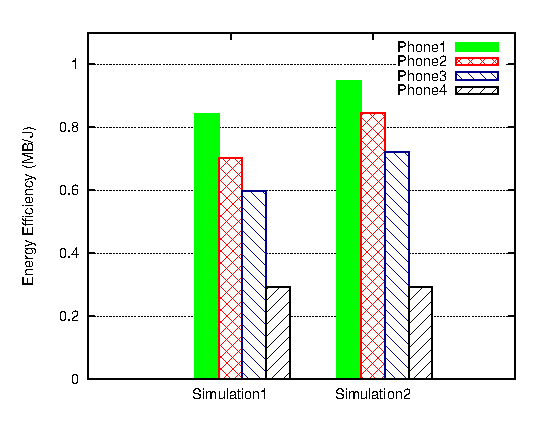
\includegraphics[scale=0.85]{energy_efficiency.eps}
\caption{Energy efficiency of the 4 phones in Simulation1 and Simulation2}
\label{energy_efficiency}
\end{figure}
We define the energy efficiency as 
the fraction of the size of file downloaded and the energy consumed, given as:
$$ 
EnergyEfficiency = \frac{SizeOfFileDownloaded}{EnergyConsumed}	
\eqno(9)
$$
The energy efficiency of the four phones are illustrated in Figure \ref{energy_efficiency},
which shows that Phone1 outperforms the others phones.
In both simulations, Phone1 achieves more than 100\% energy saving compared to 
Phone4.
We further analyze why Phone1 outperforms Phone2.

In Simulation1, 
Phone2 has 13.5\% more download sessions than Phone1. This rate increases to 18.8\% in Simulation2. More download sessions
mean more actions of starting or stopping downloading files, thus wasting energy consumption in 
closing (and reestablishing) TCP connections. 
At the same time, in Simulation1, Phone1 also has 14.7\% longer average download session length than Phone2. 
In Simulation2 this rate is 21.4\%. 
These two factors contribute to the better performance of Phone1 in preference to Phone2.
We conclude that our algorithm is effective in energy saving and succeed in 
leveraging the variations of Rssi.

\section{Conclusion} 
In this letter, we first investigate the relationship between Rssi and energy consumption of smartphones
and then propose an Rssi-aware Wi-Fi download management algorithm for energy saving.
Through Monte-Carlo simulations, we demonstrate that the algorithm is effective 
since it leverages some main properties of Rssi and takes into account
tail energy of Wi-Fi. 
\section*{Acknowledgment}

This work is supported by the National Nature Science Foundation of China, NSFC (Grant No. 61170293) 
and the International Science \& Technology Cooperation Program of China, 
Ministry of Science and Technology of China (Grant No. 2014DFG12370).

\ifCLASSOPTIONcaptionsoff
  \newpage
\fi
\begin{thebibliography}{0}
\bibitem{biblio1}
Noah Pritt, \emph{Indoor Positioning with Maximum Likelihood Classification of Wi-Fi Signals}, 
\hskip 1em plus
  0.5em minus 0.4em\relax SENSORS 2013 IEEE, November 2013, p1-p4

\bibitem{biblio2}
Doug Rosener, \emph{Decreasing Rssi Setting Time in Low-power Mode Systems}, 
\hskip 1em plus
  0.5em minus 0.4em\relax US Patent, Pub.No: US 2013/0029607 A1, Pub.Date: Jan 31, 2013  
  
\bibitem{biblio3}
Frank Vanheel et al., \emph{Automated linear regression tools improve RSSI WSN localization in multipath indoor environment}, 
\hskip 1em plus
  0.5em minus 0.4em\relax Journal on Wireless Communications and Networking, 2011
  
\bibitem{biblio4}
Jenq-Shiou Leu, Nguyen Hai Tung, and Chun-Yao Liu, \emph{Non-Parametric RSS Prediction Based Energy Saving Scheme for Moving Smartphones}, 
\hskip 1em plus
  0.5em minus 0.4em\relax IEEE Transactions on Computers, July 2014, p1793-p1801
   
\bibitem{biblio5}
Monsoon Power Monitor, \emph{www.msoon.com/LabEquipment/PowerMonitor} 
\hskip 1em plus
  0.5em minus 0.4em\relax 

\bibitem{biblio6}
Di Zhang et al., \emph{Leveraging the Tail Time for Saving Energy in Cellular Networks},
\hskip 1em plus
  0.5em minus 0.4em\relax IEEE Transactions on Mobile Computing, July 2014, p1536-p1549  
  
\bibitem{biblio7}
Jian Li et al., \emph{Application-Centric Wi-Fi Energy Management on Smart Phone}, 
\hskip 1em plus
  0.5em minus 0.4em\relax  Network Operations and Management Symposium (APNOMS), 2012 14th Asia-Pacific   
 
\bibitem{biblio8}
Halton Sequence, \emph{en.wikipedia.org/wiki/Halton\_sequence} 
\hskip 1em plus
  0.5em minus 0.4em\relax  

\bibitem{biblio9}
Lashkari, A. H., Parhizkar, B., \& Ngan.  \emph{WIFI-based indoor positioning system},
\hskip 1em plus
  0.5em minus 0.4em\relax Proceedings of the IEEE ICCNT 2010, 23–25 April, 2010, p.76–78

\end{thebibliography}
\end{document}


